\chapter{基于脉搏波的子痫前期识别分析软件系统的设计与实现}
\section{引言}
本研究此前各章中均涉及了一定的软件设计与算法设计,在这些工作的基础上,本章介绍了一款基于PPG信号的PE识别分析软件系统的设计与实现过程。在分析具体功能需求后,
选取跨平台客户端+云服务器的方案进行整体设计,以期完成以下四部分内容:PPG信号的预处理与特征计算生成;PE识别模型的本地化训练与生成;跨平台的多客户端软件设计;
云服务器端软件设计与PE识别模型的部署。本章对其中涉及的软件与算法开发设计进行了详细的介绍,同时也展示了各工作内容的实现效果,
并对软件系统进行了功能性的验证与测试。

本章研究内容的框架图如\autoref{fig:frameworks6}所示。

\begin{figure}[htbp]
    \centering
    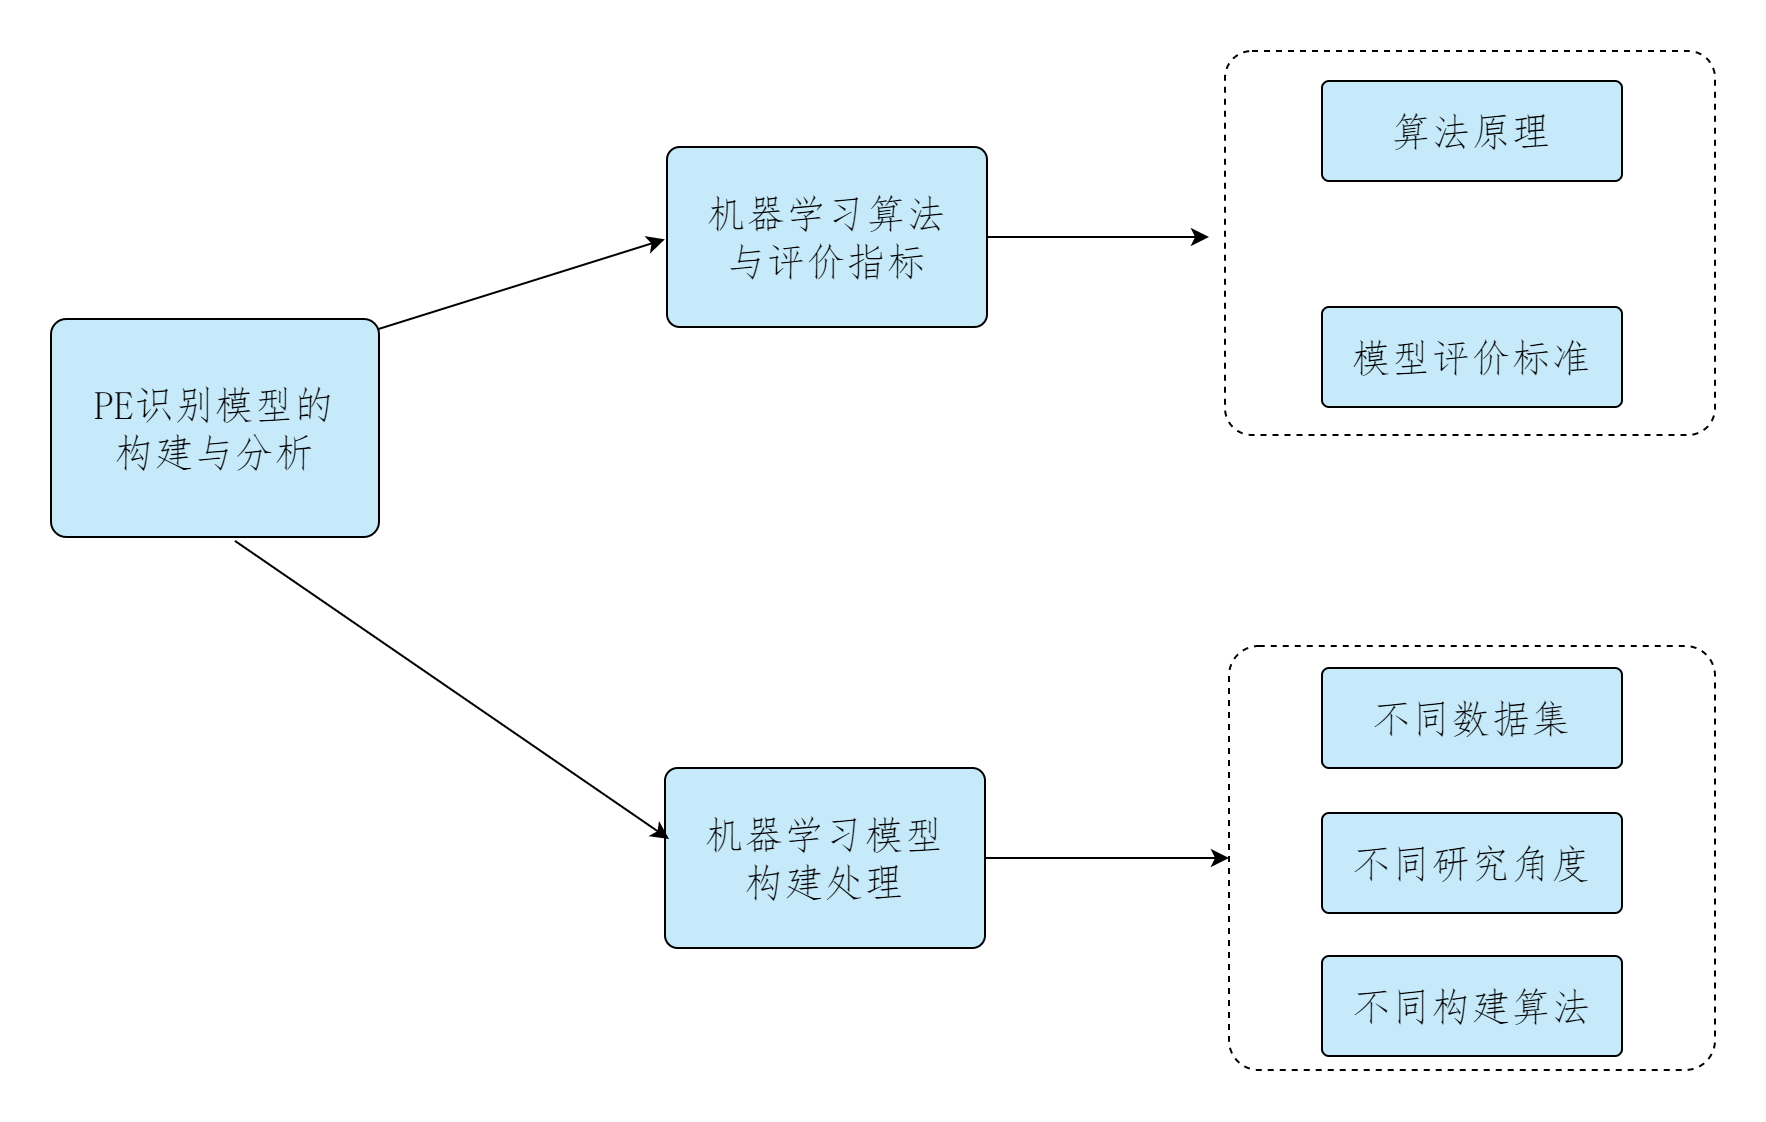
\includegraphics[width=0.9\linewidth]{results/frameworks5}
    \caption{\label{fig:frameworks6}第六章研究内容框架图}
\end{figure}

\section{需求分析}
如本研究中绪论中所介绍的,尽管移动智能医疗与可穿戴式设备已经取得了长足的发展,但现阶段PE的微型化智能化检测技术仍处于起步阶段,国内外相关研究匮乏。
而由于PE的高危害性,实现PE的早期检测识别诊断无疑可以极大地保证孕妇及婴儿的生命健康安全。因此,设计实现一款可以满足实验室研究、医院监护、社区检查、
居家监护的多应用场景的PE识别诊断软件综合系统无疑有着巨大的市场前景,具有极大的临床意义。另一方面,上述软件系统在保证完整分析功能的基础上,
应支持软件自身更新迭代导致的各种变化。这要求软件系统在开发伊始就需要进行考虑不同的开发与应用情景,引入软件开发的
代码复用与模式设计等技术,增加软件系统的健壮性与复用性\cite{Enrich2018}。

因此,软件系统需要满足以下具体需求,并根据实际需要,进行一定的兼容性设计:

一、核心分析功能完整

软件系统需具备完整的PE分析功能,包括不限于对原始数据进行预处理、提取计算相关特征、构建分析数据集、对数据集进行清洗、特征提取、
识别分类模型训练和生成及最后对新数据进行预测分类等。

二、可更新迭代的处理算法

在上述软件系统的核心分析功能的各环节中均会涉及到一定的处理算法,如数据预处理时的滤波检波算法、特征提取时的各种新型参数的计算算法以及识别模型的机器学习训练生成算法等。
软件系统需要支持对以上算法的更新与迭代,避免由于算法的调整、切换、更新、迭代等操作引发大量的代码修改与重构等问题的出现。

三、可动态调整的识别模型

在第五章已经介绍过,多种机器学习算法均在PE的识别分析中得到了应用。软件系统需要支持对这些由不同算法生成的不同识别模型的切换,
针对需要预测的新数据,保证返回对应模型的预测结果。

四、有效的数据管理

由软件系统的核心功能分析可知,除最基本的原始数据外,系统还需要对基于原始数据的二次提取特征参数、数据集划分结果、PE识别模型的训练参数及模型本身等多种数据进行管理。
如何高效、有序的管理各类原始数据及中间数据也是软件系统需要解决的问题之一。

五、云服务器+跨平台客户端

软件系统需要充分考虑到多种满足在实验室研究、医院监护、社区检查、居家监护多种场景下不同的使用需求。因此,云服务器+客户端无疑是最优的解决方案,而考虑到智能便携式设备的普及,
PC端与移动端均需开发对应的客户端。

六、完备的日志记录

软件系统需要具有完备的日志记录功能,方便在开发或部署之后,随时定位、调试可能出现的问题。由于软件系统模块繁多、功能齐全,如果没有完备的日志记录功能,
软件系统的debug过程将举步维艰,同时,也很难评估软件系统的运行状态。

七、数据源兼容性

软件分析系统的使用的原始数据可能来自多种硬件采集设备自行采集或公开数据库。对于采集得到的数据,不同硬件设备使用的电子元器件、传感器等在性能参数上的区别可能导致
采集得到的数据在信号质量、采样率、分辨率及数据存储与解析格式等方面均存在差异。而由数据库得到的数据,其字段信息也极容易出现差异。保持对不同数据源的兼容性
也是软件分析系统需要重点解决的问题之一。

八、其他拓展性

基于本研究此前章节相关内容,软件分析系统使用PPG信号作为原始数据输入。但随着高性能的数据采集设备的普及,同时使用多通道多参数生理信号(如ECG、BCG、EEG)
也存在着联合分析的可能,需要软件分析系统进行一定的兼容性设计。此外,尽管软件分析系统是为PE的识别分析为初衷进行设计,其核心分析功能可作为类似研究的参考模板,
软件分析系统在进行设计时也可以考虑整体的移植性。

\section{总体设计}

根据上小节中需求分析的相关内容,最终实现的软件分析系统按照低耦合、高拓展的原则进行了模块化、功能化的设计,
每一模块只处理某一类特定任务,以实现功能高内聚性,并保持模块间的松耦合性。

一、模块化设计

软件分析系统整体设计框图如\autoref{fig:scas}所示。上小节中提及的软件系统的核心分析功能被拆分为四个独立的功能模块分别实现,以下为具体介绍。
% \begin{figure}[htbp]
%     \centering
%     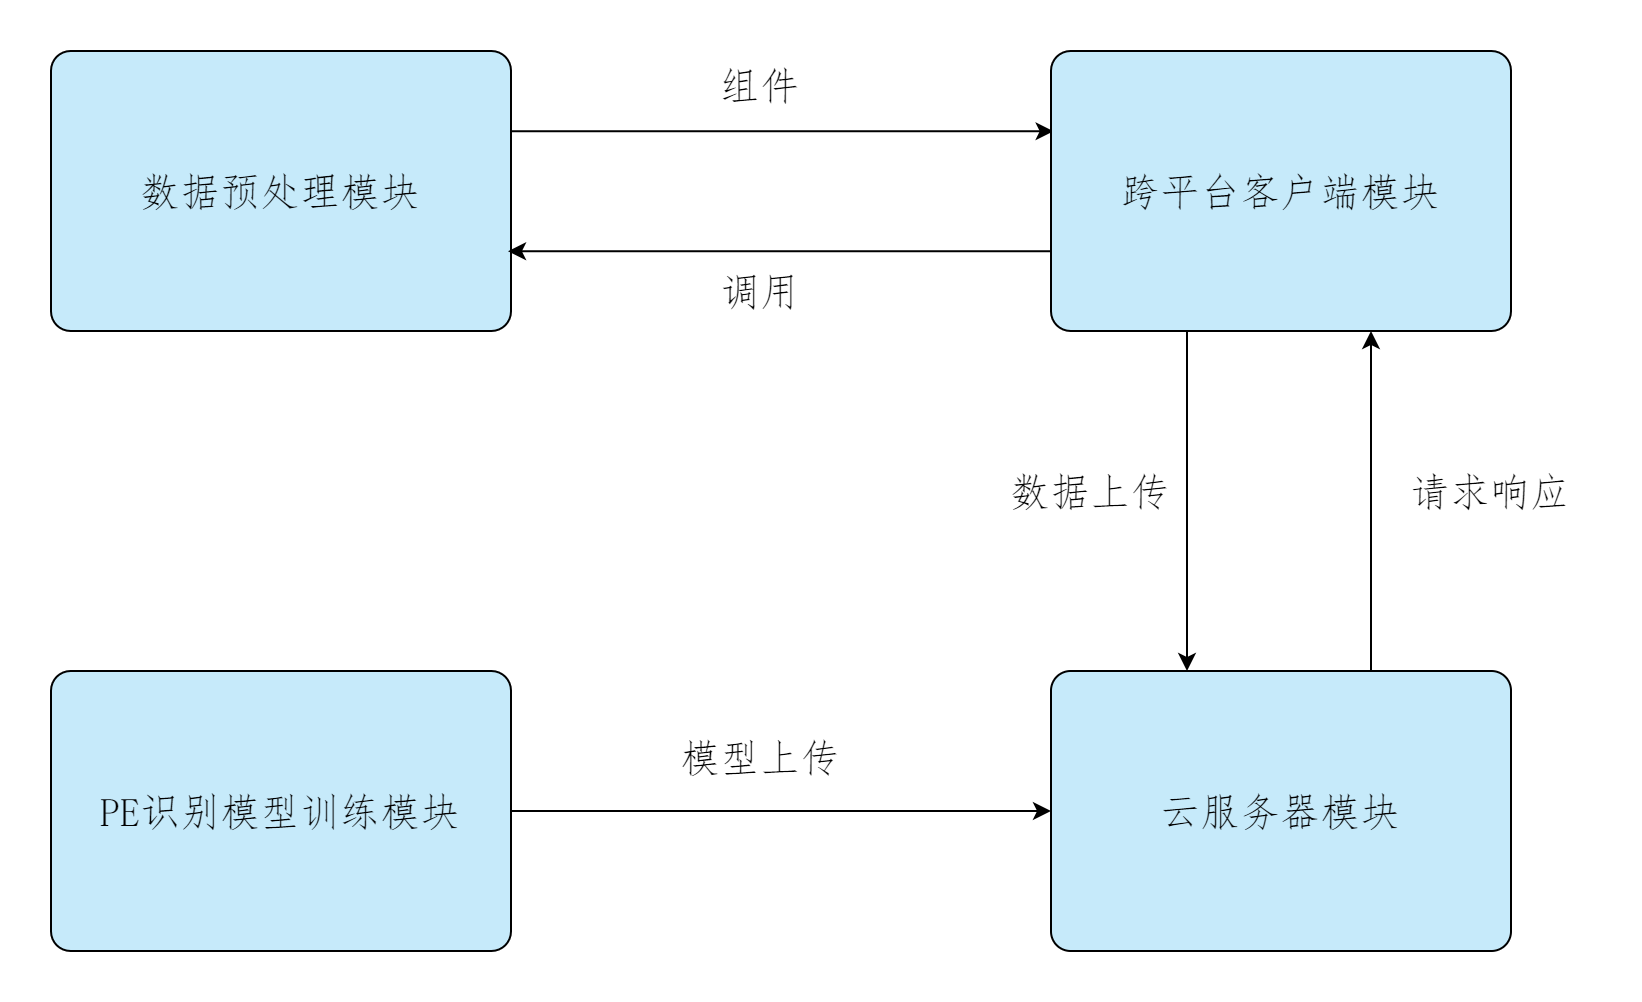
\includegraphics[width=.6\linewidth]{ch6/scas}
%     \caption{\label{fig:scas}软件分析系统设计框架}
% \end{figure}

1、数据预处理模块

数据预处理模块主要负责从原始PPG信号中提取数据特征,包括数据的读取、PPG信号的滤波降噪、波形的检测识别、特征定义及计算等处理任务。
数据预处理模块的各项处理算法或处理步骤需具有稳定性,不依赖具体部署的平台或应用场景。在此前第三章中介绍过的SCD算法也在数据预处理模块涵盖范围内。

2、跨平台客户端模块

为在多种平台下使用本软件系统,跨平台客户端模块需要完成所需操作平台下的客户端的开发。上述数据预处理模块直接在客户端模块中得到调用,PPG波形的特征数据经客户端
经由互联网被发送至云服务器端进行处理分析,云服务器的处理分析结果也会经由互联网发送返回给客户端进行展示。

3、PE识别模型训练生成模块

在获取客户端发送来的数据后,PE识别模型训练生成模块需要选择合适的机器学习算法基于这些输入数据训练生成PE识别模型,模型在训练过程中所使用的具体数据集、初始参数及调整优化后
的超参数需要同时被记录保存。生成得到的PE识别模型最终需要被部署在云服务器上,为后续新数据进行预测分析。

4、云服务器模块

云服务器模块负责管理由客户端发送来的数据信息、管理系统具体PE识别模型。当客户端发来新的数据并请求分析时,云服务器模块从客户端发送来的参数信息中确定具体使用的识别模型,
将数据交由对应的模型进行分析后,将分析结果返回至发出请求的具体客户端。

二、设计原则的应用

为使具有以上功能的多模块化软件系统的开发能顺利进行,在开发过程中必须借助计算机软件开发领域的相关思想,遵循一定的开发原则。

1、面向对象编程

面对对象编程(Object Oriented Programming,OOP)是一种计算机编程架构,尽可能模拟人类的思维方式,使得软件的开发方法与过程尽可能接近人类认识世界、
解决现实问题的方法和过程。OOP使得描述问题的问题空间与问题的解决方案空间在结构上尽可能一致,把客观世界中的实体抽象为问题域中的对象。
借助OOP的抽象、继承、多态等特性,可以简化复杂的编程过程,使软件开发的逻辑更为简单。

2、设计模式

设计模式(Design Pattern,DP)是计算机软件设计中对某些特定问题的优化解决方案的总结。DP是一套被反复使用、多数人知晓的、经过分类编目的、代码设计经验的总结。
在程序开发过程中使用设计模式,可重用代码、让代码更容易被他人理解,保证代码可靠性的同时也增加了程序的重用性。

三、编程语言与开发环境

软件系统各模块所使用的编程语言与开发环境工具如\autoref{tab:ides}所示,模块所使用的一些重要组件或开源库也在表格中进行了说明。

\begin{longtblr}
    [
        theme                   = {zju},
        caption                 = {不同模块使用的编程语言与开发环境汇总},
        label                   = {tab:ides},
    ]
    {
        width                   = \linewidth,
        colspec                 = {X[1,c,m]X[1.8,c,m]X[1,c,m]X[1,c,m]X[2,c,m]X[1.5,c,m]X[1.5,c,m]},
        hline{1,Z}              = {\thickline},
        hline{2}                = {\thinline},
        rowhead                 = 1,
        row{3,4,6}              = {bg=\oddcolor}, 
        row{2,5}                = {bg=\evencolor},
        row{1}                  = {font=\headfont,bg=\headcolor},
        row{2-Z}                = {font=\nonheadfont},
        cell{3}{1-2}            = {r=2,c=1}{c,m},
    }
    序号 & 模块 & 平台 & 开发语言 & 版本 & 开发工具 & 其他组件或库 \\
    1 & 数据预处理 & / & Java & OpenJDK(16.0.2) & VS Code & / \\
    2 & 客户端 & PC & Java & OpenJDK(16.0.2) & VS Code & / \\
    2 & 客户端 & Android & Java & Android Studio default JDK(11.0.12)  & Andoird Studio & / \\
    3 & 模型训练 & / & Python & 3.9.7 & PyCharm & Sklearn \\
    4 & 云服务器 & / & Python & 3.9.7 & PyCharm & Django、Sklearn \\
    
\end{longtblr}

软件系统的数据预处理模块与客户端模块使用Java语言开发完成。
作为一种高级语言,Java兼具解释型编程语言与编译型编程语言的特性,是目前最流行的面向对象语言之一\cite{Li2015}。
除一般面向对象编程语言的抽象继承等特性外,Java还支持抽象类、接口等设计,可以满足上述此前需求分析中的各项具体内容。
Java具有出色的跨操作系统平台特性,可以实现一次编译、多处使用。除PC端外,Java同时也是移动操作系统Android的主力开发语言之一\cite{android}。
鉴于Java的种种优点,因此,软件系统的数据预处理模块与PC客户端模块最终选择了Oracle开源版本的OpenJDK(16.0.2,GPLv2协议)\cite{openjdk}在VS Code集成开发环境
(Integrated Development Environment,IDE)下开发完成;
而Android客户端则选择了Android Studio作为IDE,使用Android Studio自带的Java版本(11.0.12,Apache协议)完成开发。


软件系统的模型训练模块与云服务器模型使用Python语言开发完成。
Python是一种高层次的结合了解释性、编译性、互动性和面向对象的脚本语言,是近年来最为流行的编程语言。
Python开源、免费、易学,也具备极强的可移植性,可以非常方便地部署在不同的操作系统与平台下。
此外,Python有着非常丰富的库组件,包括科学计算与人工智能领域极为有名的NumPy、SciPy、Sklearn与TensorFlow等组件。
因此,软件系统的模型训练与云服务器模块均选择了开源的Python(3.9.7,GPL协议)在PyCharm IDE下开发完成。
此外,云服务器模块还选取了基于Python的Django为Web框架完成服务器端相应功能的开发,选择了MySQL作为数据存储的数据库。

\section{模块设计}

针对需求分析中提出的多项具体要求,本小节将具体介绍总体设计中确定的四个模块的设计与开发过程。
\subsection{数据预处理模块}

数据预处理模块的处理流程如\autoref{fig:preprocess2}所示。下面依次介绍各流程的详细设计。
\begin{figure}[htbp]
    \centering
    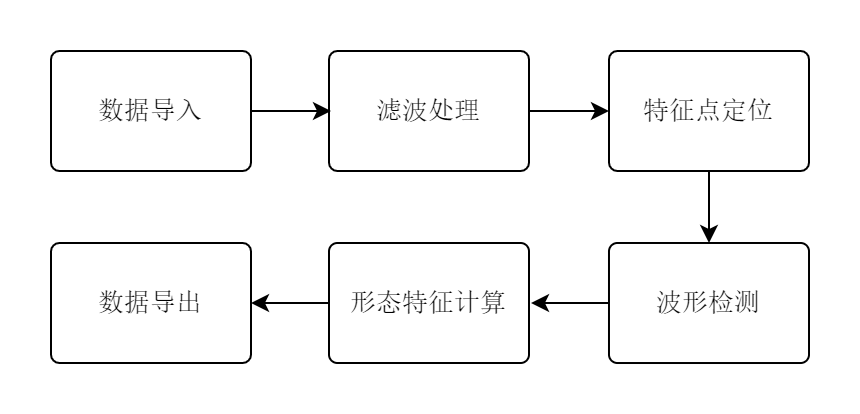
\includegraphics[width=.65\linewidth]{software/preprocess}
    \caption{\label{fig:preprocess2}数据预处理模块流程图}
\end{figure}

一、数据导入

为保持对来自不同硬件设备采集的原始数据保持读取的兼容性,软件系统使用了DP中的模板方法对这一过程进行了设计。
模板方法的基本原则是预定义一个操作中算法的骨架,而将延迟实现其中的关键步骤。
软件系统在数据读取过程所对应的抽象基类中定义了模板方法,并在模板方法中定义了数据读取过程的操作骨架,如\autoref{fig:template}所示。
基类中的读取方法被定义为抽象方法,真正的业务方法必须在基类的具体子类中实现。
当主程序需要读取数据时,只需实例化特定子类后,在子类中调用上述模板方法。
由硬件差异、数据格式等原因导致的读取方法的差异可以在读取过程的不同子类中实现。
这种机制延迟实现了读取的具体处理过程,隔离了数据读取功能对系统其他功能的影响,也保证了系统整体的灵活性。
在这种设计下,目前软件系统已经支持对GE、迈瑞ePM 15M生理信号监护仪等多种医用监护仪导出的数据的读取,同时也支持研究团队自研的多生理参数采集设备的数据读取,如\autoref{fig:data_sources}所示。

\begin{figure}[htbp]
    \centering
    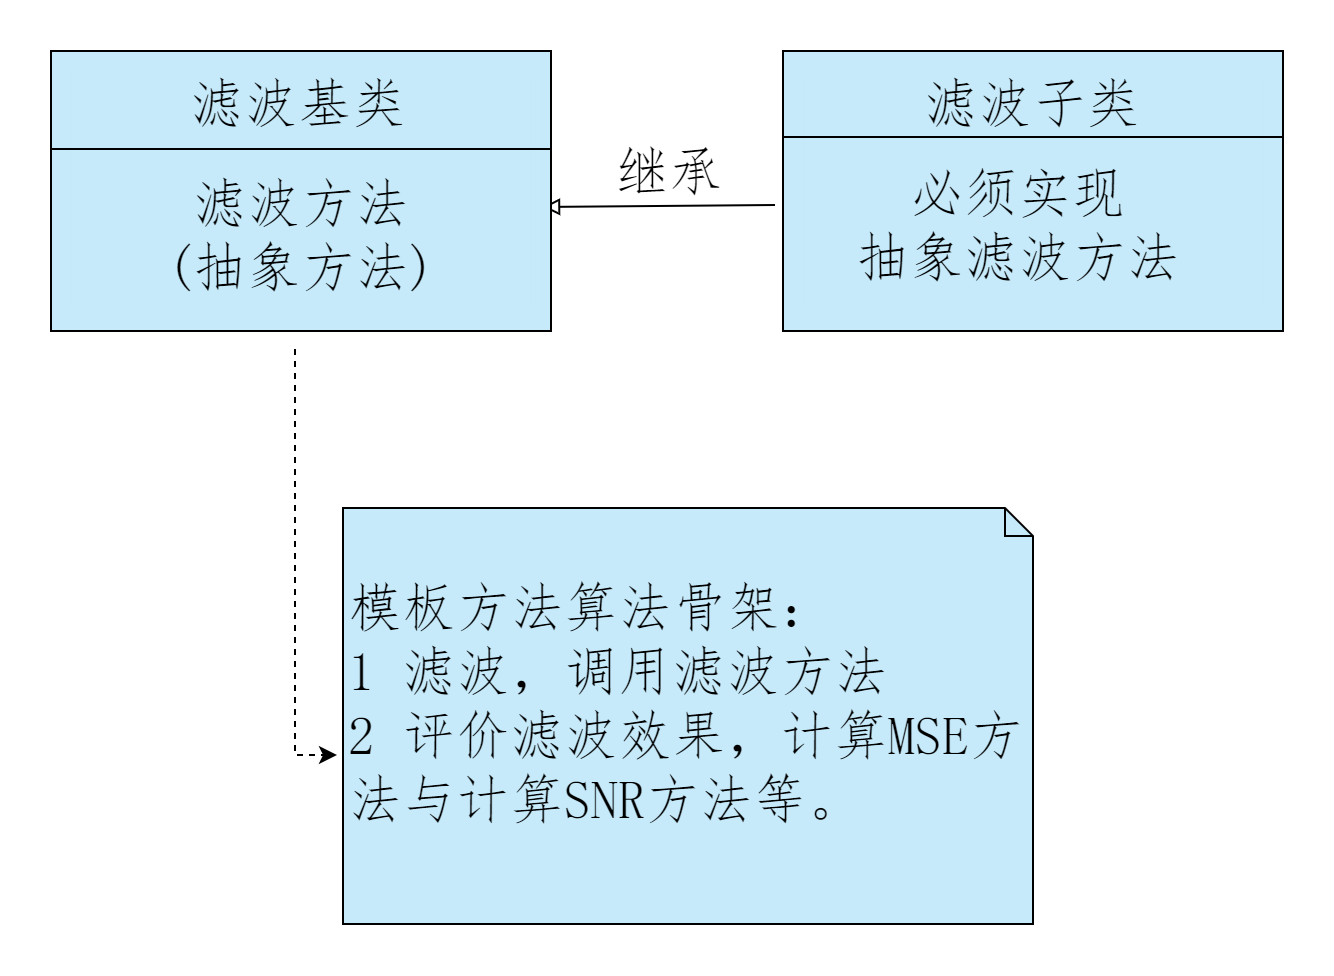
\includegraphics[width=.65\linewidth]{software/template}
    \caption{\label{fig:template}数据预处理模块流程图}
\end{figure}

\begin{figure}[htbp]
    \centering
    \subfigure[GE B650监护仪]{
    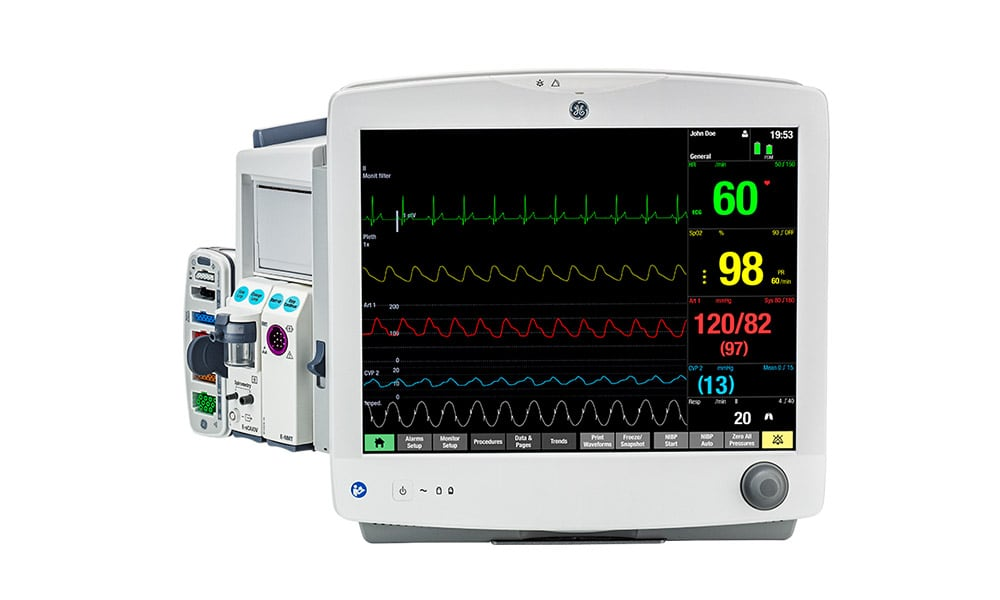
\includegraphics[width=5.5cm]{pulse_preprocess/monitor1}
    }
    \quad
    \subfigure[迈瑞ePM 15M生理信号监护仪]{
    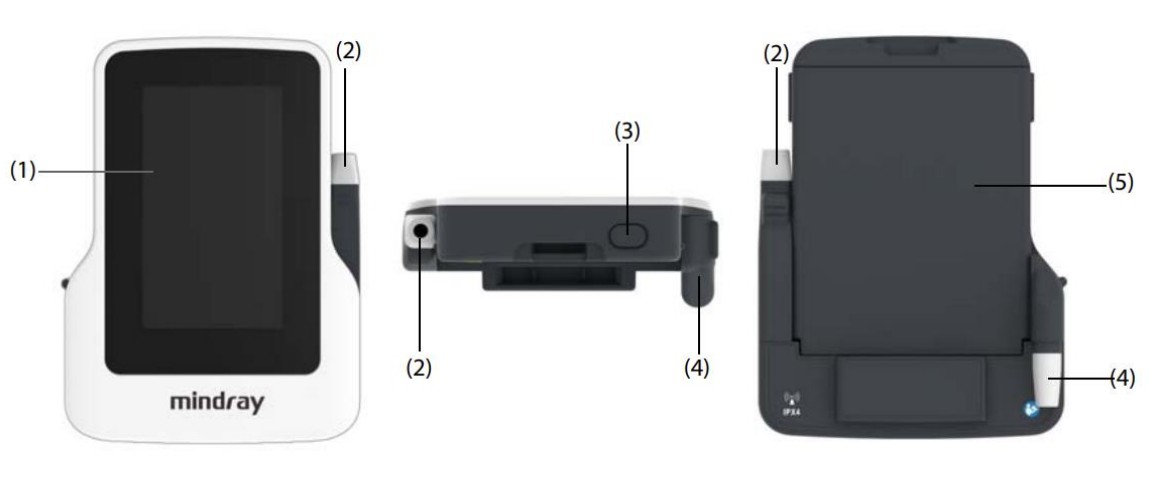
\includegraphics[width=5.5cm]{software/ep20}
    }
    \quad
    \subfigure[研究团队自研的多生理参数采集设备]{
    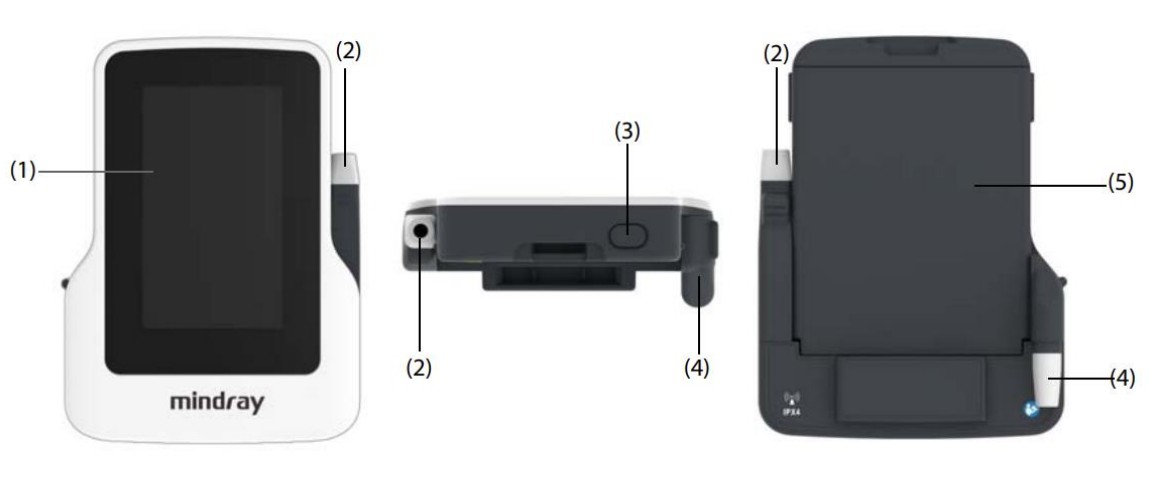
\includegraphics[width=5.5cm]{software/ep20}
    }
    \caption{\label{fig:B·R·A·H·M·S}德国Thermo Fisher Scientific公司的KRYPTOR检测设备}
\end{figure}

\subsection{跨平台客户端模块}


\subsection{PE识别模型训练生成模块}


\subsection{云服务器模块}


\section{测试与验证}
\section{小结}


一、客户端模块

客户端模块即数据准备模块,负责绝大部分数据处理任务,包括对数据的读取、预处理、特征计算等工作。数据处理完成后以Json的存储格式上传至服务器端,并根据上传时选择参数,由服务器训练好的数据模型返回相应的PE预测分类结果。
为方便对移动智能平台的支持,客户端模块采用静态面向对象语言Java编程完成。

二、模型训练模块

模型训练模块是软件系统的核心算法模块,需要基于提取好的数据特征完成所有模型训练、分类处理工作。由于Python在机器学习领域的广泛普及,此模块的所有编程设计与实现全部基于Python完成。训练好的分类模型也会部署至服务器端。

三、数据存储模块

数据存储模块即服务器模块,是上述两个模块的中间件,接收来自客户端的特征等数据,并将相关数据存储至数据库中,同时根据相应的特征值依据训练好的模型给出相应的预测结果。为能直接使用由模型训练模块生成的多种机器学习模型,数据存储模块采用Python为
主要编程语言,。


\section{模块具体设计与实现}
\subsection{客户端模块}


一、多种来源的数据格式的支持

本研究开展时,所有数据均来源自GE设备balabala,数据是以csv格式导出的。在研究后期,课题组也引入了迈瑞公司的 。与此同时,课题组自研多生理信号采集终端也已完成,最多可支持对127路生理信号的采集,如\autoref{fig:msd}所示。
不同厂商的硬件设备的采集得到的数据可能会有采样率、采样精度的差异,同时导出数据项也往往不尽相同。显然综合软件系统的数据读取功能需有一定的硬件适配性,
可以依据数据通讯协议、存储格式的不同灵活定制,以实现对多种硬件设备的兼容。
% \begin{figure}[htbp]
%     \centering
%     \subfigure[连接实物图]{
%     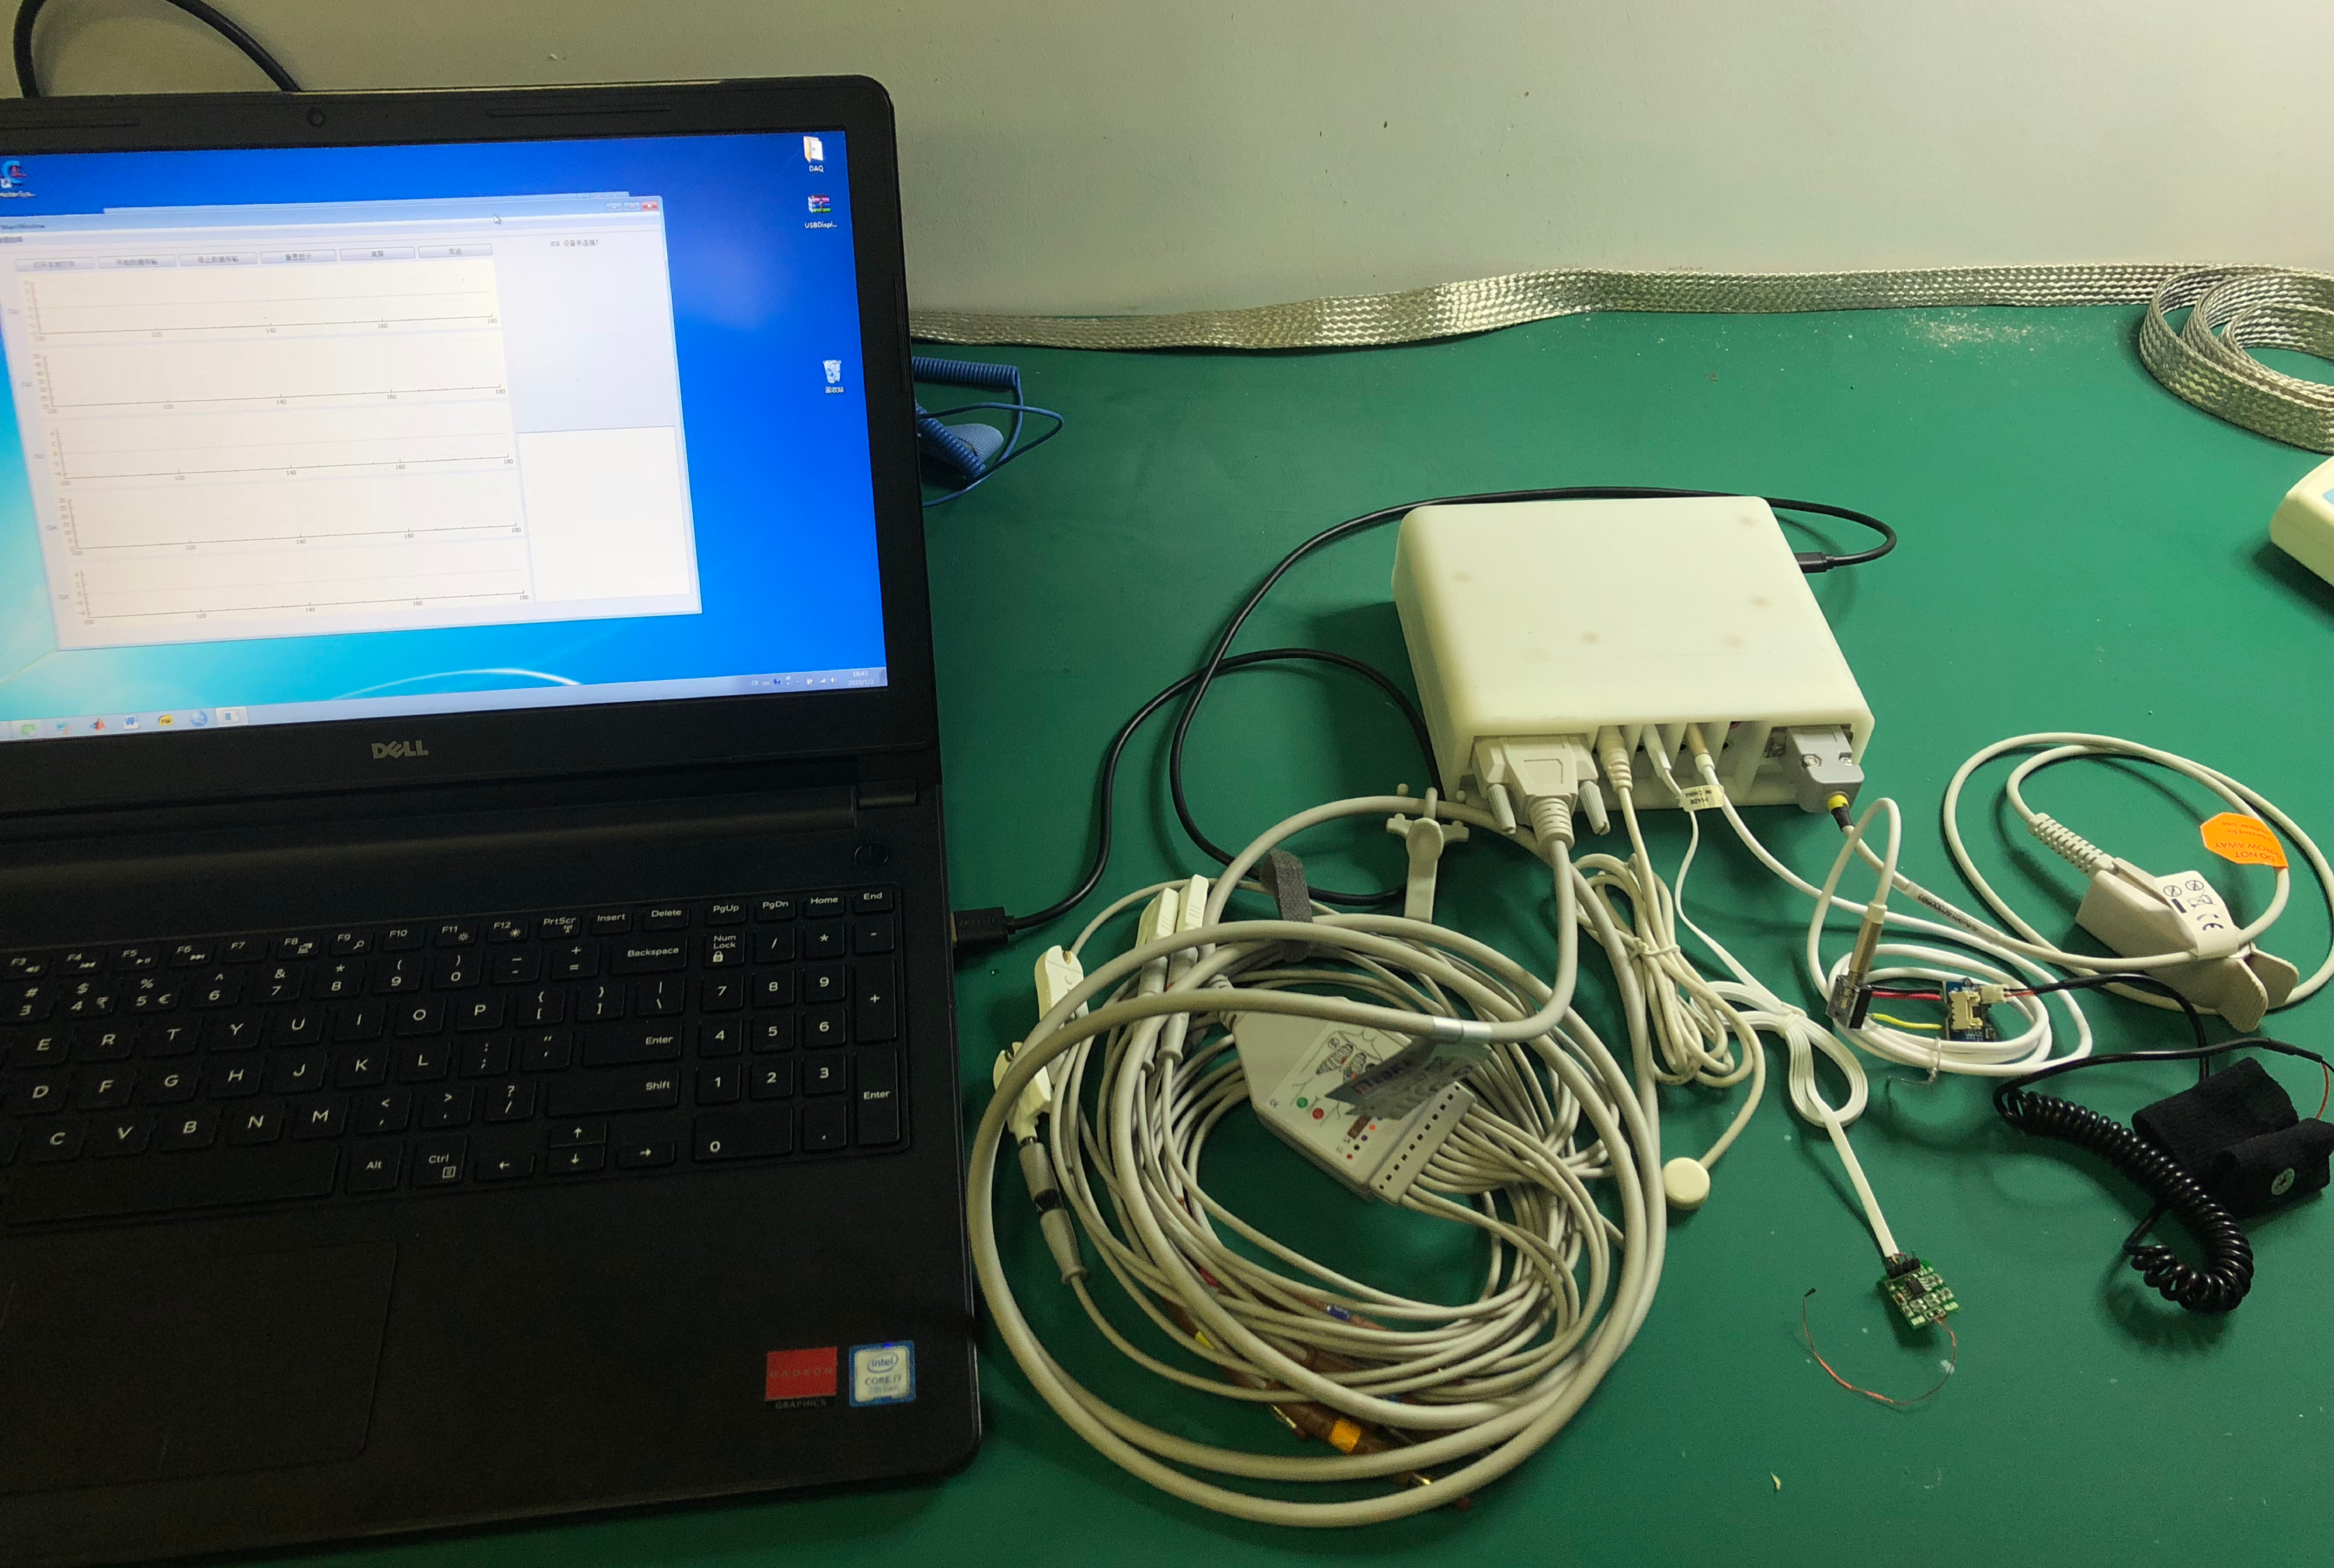
\includegraphics[width=5.5cm]{ch6/SystemCon}
%     }
%     \quad
%     \subfigure[采集得到的信号]{
%     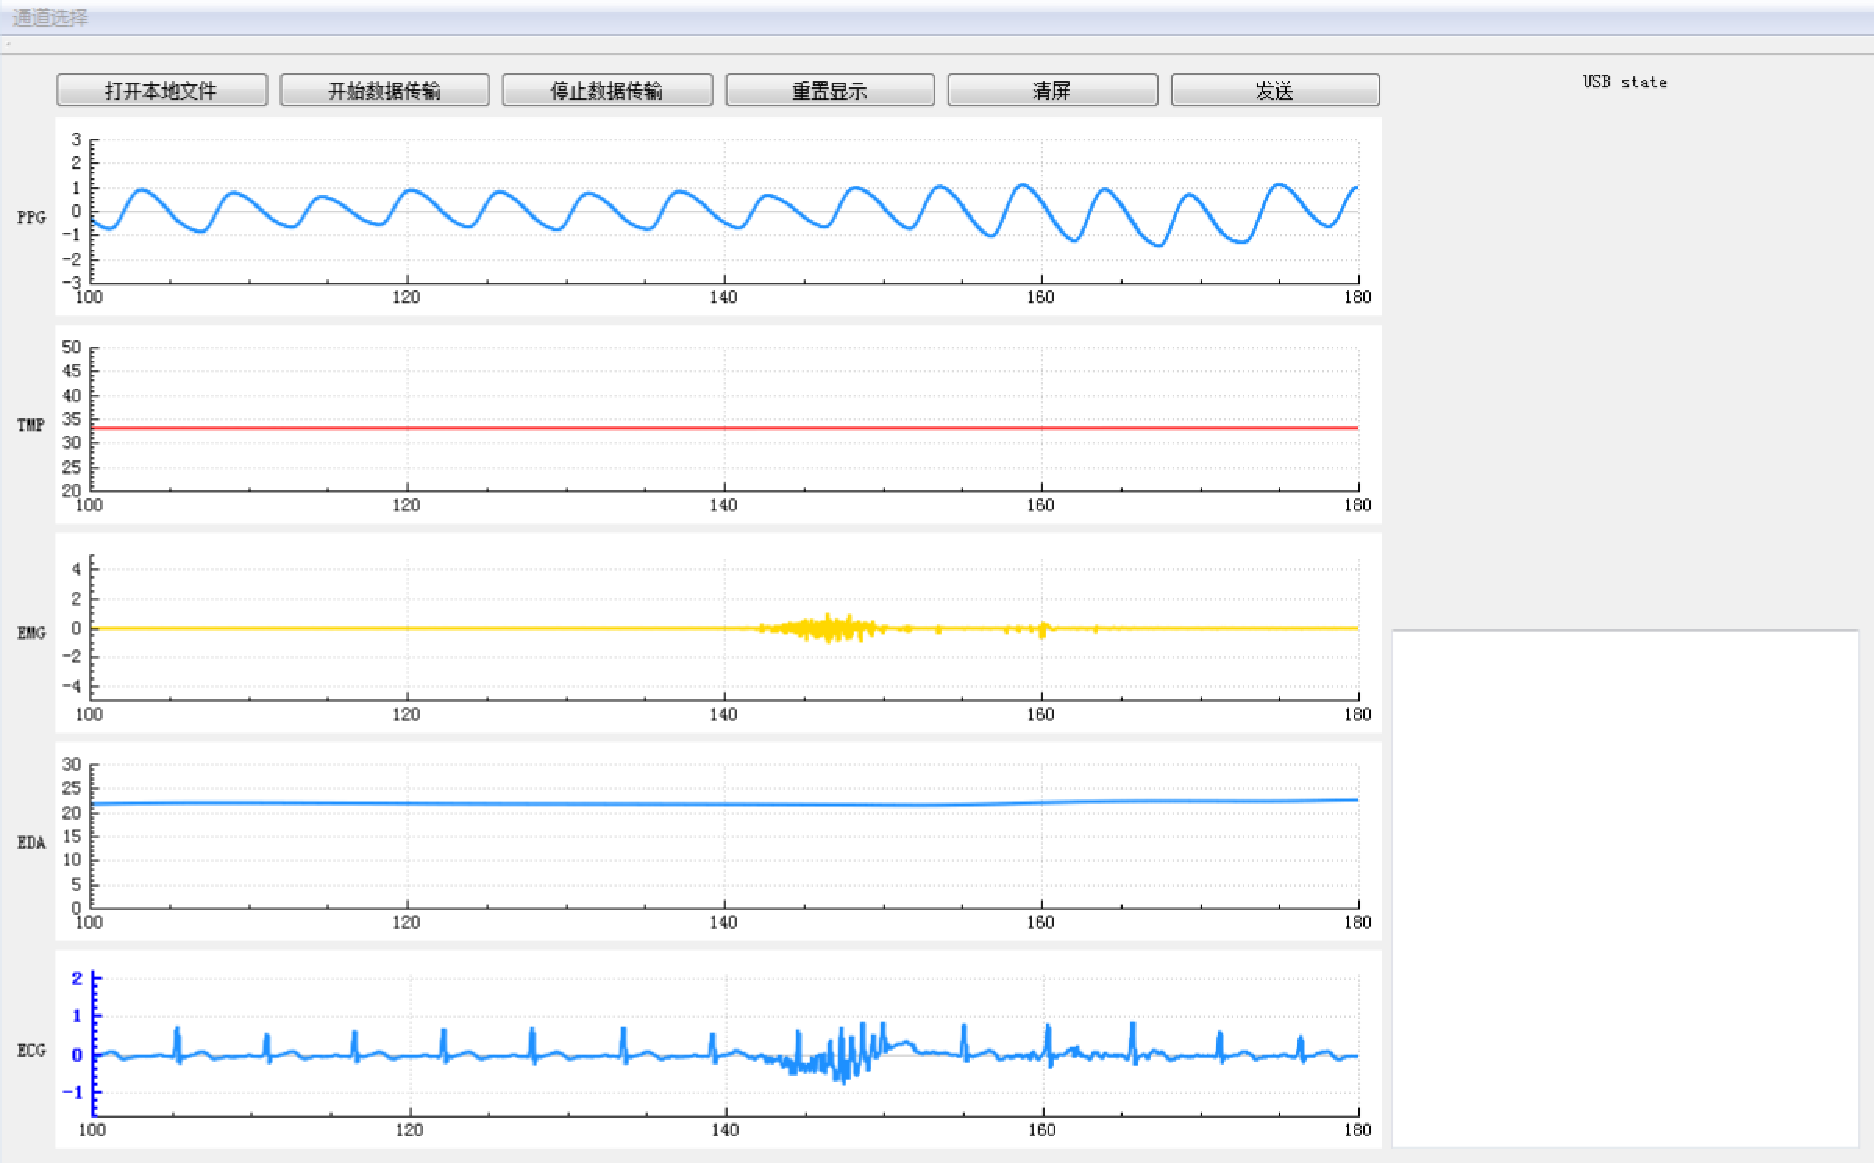
\includegraphics[width=5.5cm]{ch6/data}
%     }
%     \caption{\label{fig:msd}课题组自研多生理信号采集终端}
% \end{figure}

为隔离由于不同硬件数据格式给数据读取模块带来的变化,在综合软件分析系统的设计中使用了规范与实现分离的机制,利用Java接口完成了所需功能。具体实现是首先将数据读取的过程定义为一抽象接口$PPGReader.class$。由于接口无法实现具体方法,因此,
当来源自某种硬件设备的数据需要进行读取时,需要一个特定的子类$SpecificReader.class$去继承该抽象接口并具体实现读取的$readFromFile.class$方法。当实现好多个与硬件绑定的子类后,需要在$TotalReader.class$类中真正读取数据时,即可按图索骥,
找到与硬件数据解析方式相对应的具体子类。这样的设计可以确保与硬件相关的特性被封装隐藏并可以随时增加新的硬件支持。这一过程中的伪代码如\autoref{lst:reader}所示。

% \lstinputlisting[caption={数据读取模块的伪代码实现},label=lst:reader,style=myJava]{code/ch6/PPGReader.java}

二、预处理算法设计

数据预处理部分的软件算法工作主要由等几部分组成。由于本小节部分内容与第四章内容较为接近,预处理工作的具体实现思路可参阅前文。而数据滤波与波形检测的软件设计均采用了策略与机制分离的思想,利用工厂设计模式\cite{Enrich2018}完成。

1. 数据滤波

如前所述,在对生理信号的进行数字滤波时,一般会涉及多种类型的数字滤波器甄选。同时,每种滤波器也会有相应的可调参数。因此,性能最佳的滤波器的选择往往需要对多种滤波器调参后综合测评后才能判别,因此,软件分析系统需要能在多种滤波器之间灵活切换。

为实现上述功能,首先定义了抽象的滤波器基类$Filter.class$,在该基类中定义了滤波器的滤波、调参等基本操作的抽象方法。其次,每种特定滤波器$SpecificFilter.class$作为子类继承并实现$Filter.class$中的所有抽象方法。所有的滤波器子类并不直接实例化
,而是通过额外定义的$FilterFactory.class$这一工厂类来实现。在$FilterFactory.class$中定义好$getFilter()$方法,在该方法中选择适当的滤波器种类,将其实例化后,根据实际需求调整好滤波器性能参数并返回该实例。另一方面,当主程序中需要使用
滤波器对原始信号进行处理时,仅需调用$FilterFactory.class$的$getFilter()$方法即可。任何对滤波器种类及相关参数的设置与修改对主程序而言均是不可见的,从而很好的隔离了滤波器设置对主程序代码的影响,降低了软件系统的耦合性。
这一过程中的伪代码如\autoref{lst:filter}所示。
% \lstinputlisting[caption={滤波器设置的伪代码实现},label=lst:filter,style=myJava]{code/ch6/PPGReader.java}

2. 波形检测

脉搏波波形检测是本研究的基础,波形检测算法的准确性将直接影响后续分析工作。此前的研究人员已经提出过多种脉搏波波形检测方式\cite{Wang2012},本文则在前人基础上进一步优化了波形检测的流程,将之前的一次性检测改成了检测-复核-决策(Detect-Check-Keep)
的反馈式检波流程,进一步提高了脉搏波波形检测准确性,该过程中的流程图如\autoref{fig:check}所示。
% \begin{figure}[htbp]
%     \centering
%     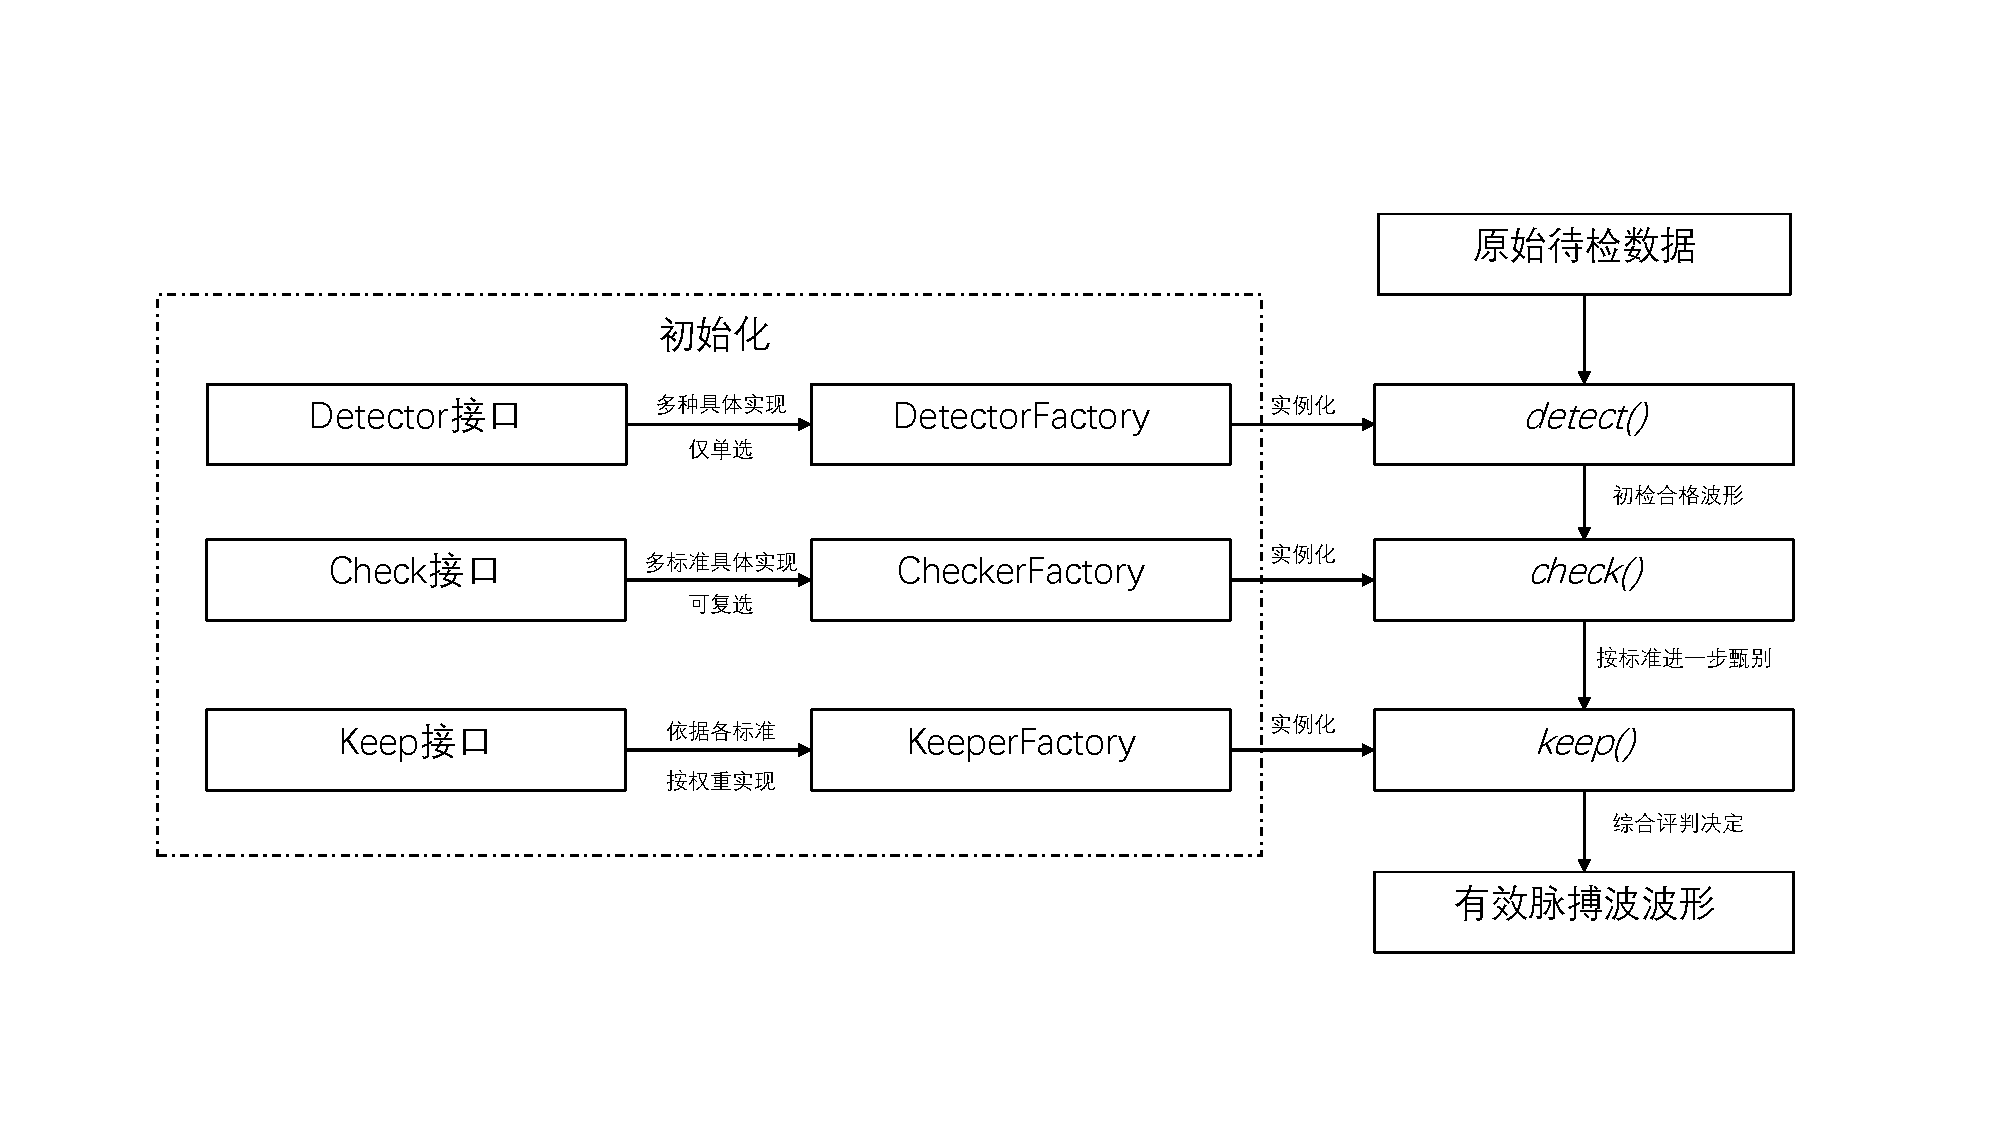
\includegraphics[width=1.1\linewidth]{ch6/check}
%     \caption{\label{fig:check}改进后的检波流程图}
% \end{figure}

其中,$detect()$方法负责按照一定的基础规则初步筛选出所有可能脉搏波波形位置。$check()$方法则遵循一定的标准,对初筛的结果进一步复核,筛选出某些不符合标准的疑似误检的波形。其中,本研究中自行定义了一些复核标准,
包括如两个波形的间期需在合理时间内、同一人的脉搏波波形在短时间内波形应较为接近、单个脉搏波波形的能量不应与所有波形的平均能量有较大的出入等。随后$keep()$方法则负责对$check()$的结果进行综合评判,可按照投票决策或比重决策等方式来决定最终判断疑似误检波形的
去留。最后,在初筛的波形中剔除误检的波形则可得到最终的检测结果。

与上小节中的数字滤波的工厂模式设计类似,Detector、Checker及Keeper分别是检波算法、复核算法及决策算法的基类,分别定义了各算法的基本行为,但不负责实现具体功能。具体的实现算法需要重新定义子类继承相应的基类,
并实现其中的相应的$detect()$、$check()$及$keep()$方法。此时,再分别定义各算法的工厂类,将各算法实例化过程进行封装。其中,需要注意的是,$DetectorFactory.class$与$KeeperFactory.class$返回的实例都仅含有一个对象,而$CheckerFactory.class$
可以返回包含多个实例的集合,即同时返回多个复核标准同时对初筛结果进行检测。

上述设计可以有效提高脉搏波波形检测的准确性,并且可以按需求灵活定制筛选标准、调整检波精度。与此同时,根据实际需要和检波效果等因素,检测算法的Detector、Checker及Keeper等部分均可自行改动、调整、优化,且不影响主程序中的代码执行,从而实现了
检波算法的各环节的高内聚性及算法与系统整体之间的低耦合性。

三、信号特征算法设计

基于脉搏波的波形检测算法无疑是客户端软件的核心功能之一,且是客户端软件中改动变化最频繁、最容易因代码的更迭而发生增删修改的部分。降低特征算法的更迭对客户端软件的整体影响,是对特征算法整体设计的基本要求。本研究中,对特征算法
的整体设计如\autoref{fig:features}所示。
% \begin{figure}[htbp]
%     \centering
%     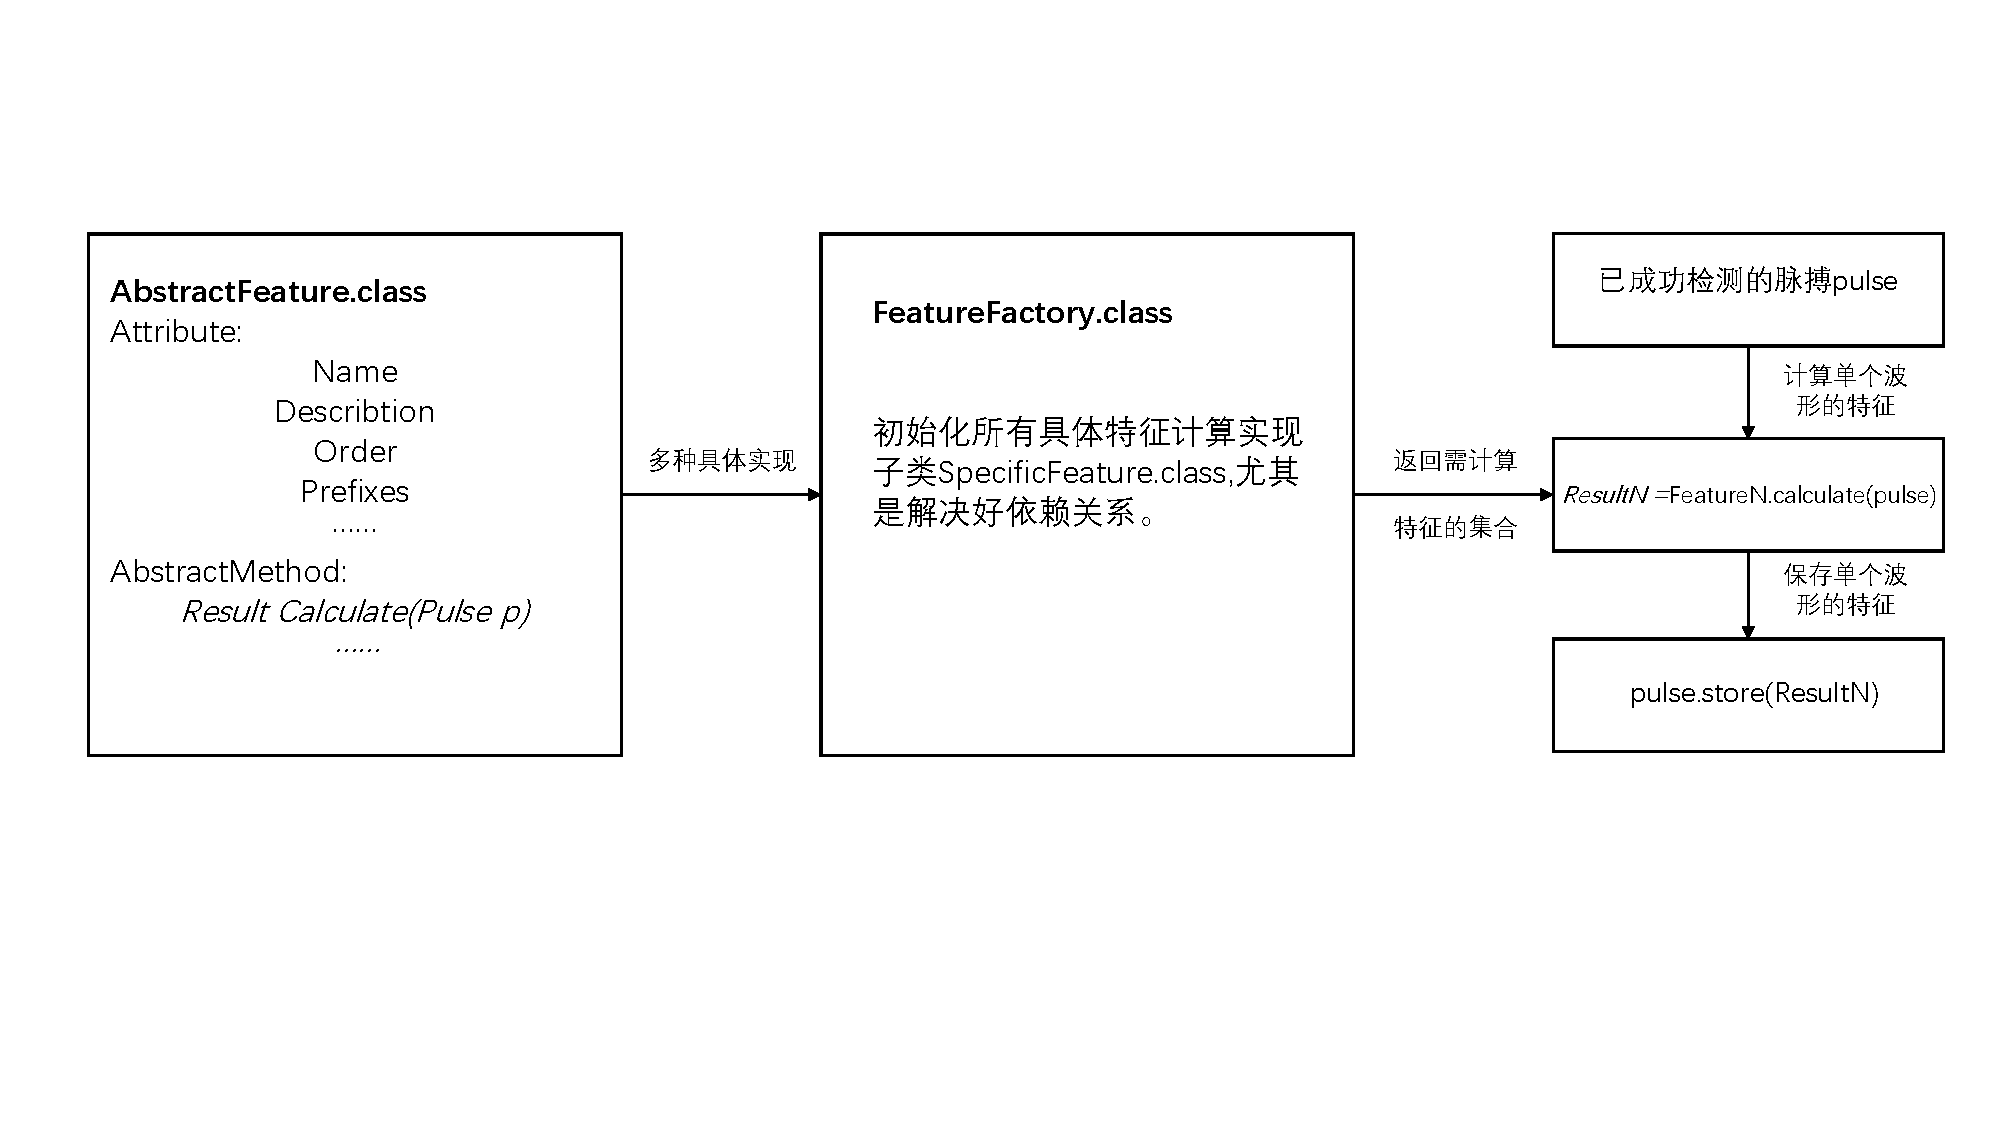
\includegraphics[width=1\linewidth]{ch6/feature}
%     \caption{\label{fig:features}特征计算的算法流程图}
% \end{figure}

与前小节的设计类似,$AbstractFeature.class$是个抽象父类,规定了所有特征应有的一般属性,包括特征名及其缩写$Name$,特征所代表的含义$Describition$等描述信息。而在$AbstractFeature.class$的子类$SpesificFeatureX.class$中才根据具体设计思想等完成对
该特征的计算过程$calculate()$。值得注意的是,在\autoref{fig:features}中,$AbstractFeature.class$额外定了两个属性$Order$与$Prefixes$。
这是因为某些特定的特征在计算时,可能需要一定的先导条件,即需要预先计算好一定的先导特征。因此,每个特征在初始化时,按照先导条件从无到有、从少到多、从简单到复杂的原则,给每个具体实现子类$SpesificFeatureX.class$设置好其计算顺序
$Order$及保存着其先导特征$Order$的$Prefixes$,最后按照所有子类$SpesificFeatureX.class$的$Order$遍历,即可保证所有特征均按指定顺序全部计算完毕。

而上述先导设置过程,可以在$SpesificFeatureX.class$定义时设定,但为了保持更多的调整灵活性。最终在实现软件系统时额外定义了$FeatureFactory.class$,用以集中完成并封装所有需进行计算的特征子类的初始化工作。而在主程序中调用$FeatureFactory.class$
的$GetAllFeatures()$方法时,其返回值将是包含所有特征子类的列表,并特征子类的$Order$值决定了该子类在返回列表里的排列顺序,即真正的执行顺序。若软件系统需要增加某一新型特征算法,只需设计新的$SpesificFeature.class$,实现其具体的计算过程,
随后在$FeatureFactory.class$设置好对应$Order$与所需的$Prefixes$等在内的初始化工作,即可完成对待检特征集的拓展。

此外\autoref{fig:features}也给出了特定脉搏波波形所有特征的具体计算流程。首先,客户端需完成数据预处理工作,获取所有待计算的脉搏波完整波形。其次,通过实例化$FeatureFactory.class$并调用$GetAllFeatures()$方法以获取所有待计算的特征集合。
随后,针对特征集合里面的每个$SpesificFeatureX.class$特征,分别调用其$calculate()$方法完成计算。此时特定波形的具体特征值仍然保持在$SpesificFeatureX.class$中,故最后,需要将结果保持至该波形对应的具体$Pulse.class$实例中,
即执行最后的$pulseX.Store(feature)$操作。另外,不难发现,$FeatureFactory.class$的实例化过程会随着待检波形的更迭而不断进行,最终会导致Java虚拟机重复创建、同时消耗系统内存资源。为减少该冗余操作,
最后客户端使用了设计模式中的Singlon单例模式\cite{Li2015}对$FeatureFactory.class$
进行了再次设计,即只可以创建一个$FeatureFactory.class$的实例,此后所有调用$FeatureFactory.class$的创建方法只会返回第一次调用时创建的实例。

四、多种数据类型的支持

尽管现阶段针对PE的研究主要基于脉搏波这一生理信号,但并不排除更多人体生理信号会增加进信号分析的可能。而上述过程中,涉及的脉搏波原始数据读取、预处理及信号特征设计与计算等过程也可以作为生理信号的一般处理过程。
鉴于此,客户端软件进一步设计了$AbstractBMESignal.class$这一抽象类来表征一般生理信号,数据读取、预处理及信号特征计算过程均设计成抽象方法,$Pulse.class$是继承该抽象类的复杂处理脉搏波信号的子类。若有其他生理信号的分析需求,可以视情况
拓展实现心电$ECG.class$、脑电$EEG.class$等,这一过程如所示。

五、数据导出

当客户端完成对生理信号的分析后,如何将分析处理结果进行保存是客户端软件最后需要解决的问题。导出的数据是以检测的PPG波形为基础,包含该波形所有形态特征。而在本研究中,多种新设计的特征参数往往是以向量的形式出现,因此最后导出的结果将会大量出现波形——
特征——向量(pulse-feature-vector)这种二级树状结构。此外信号特征算法出现引入了新的信号特征、对已有特征值数值的保存形式进行更改等更迭将会直接引起数据存储格式的变化。而常见的基于列表式的cvs、txt等对这种树状数据格式的支持较差,
需要借助新的数据储存格式来实现。

扩展标记语言(Extensible Markup Language,XML) \cite{xml,Li2016}与JavaScript对象标记法(JavaScript Object Notation,JSON)\cite{json,Crockford2006}是两种服务器端流行的数据交换格式。两者均可按照实际需求灵活定制存储规则,对较为复杂的数据结构
支持性好、拓展性强。但由于XML是基于标签描述数据的,在描述数组类型数据时,引入了大量冗余信息。而JSON则对数组类数据有着更好的支持,有着更快的读写速度与更高的存储效率\cite{Nurseitov2009}。因此,软件分析系统最终使用JSON作为数据交换格式,
而在具体实现时使用了中国阿里巴巴公司的开源JSON解析库fastjson\cite{fastjson}进行编码。最后的导出数据如\autoref{lst:json}所示,除基本数据特征外,与数据相关的文件信息及孕妇人口统计学信息也被保存至JSON文件。
% \lstinputlisting[caption={导出数据示意},label=lst:json,style=myJava]{code/ch6/out.json}
% \begin{figure}[htbp]
%     \centering
%     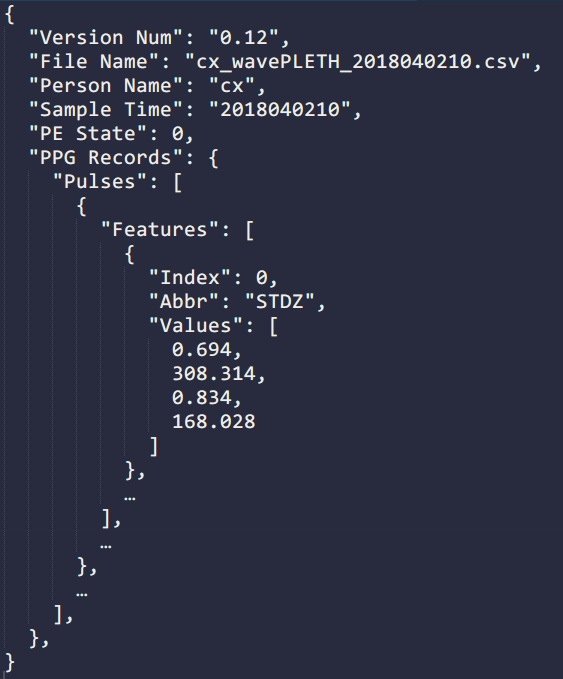
\includegraphics[width=.6\linewidth]{ch6/json}
%     \caption{\label{fig:json}导出数据示意}
% \end{figure}

六、多平台支持

综合考虑软件实际的使用场合与应用前景,本研究最终选择了对Windows PC平台及Andoird移动平台进行了适配开发。由于Java的天然的跨平台特性,前文提及的多项软件设计在实现后可直接在PC端与移动端顺利运行。另一方面,Android系统独立于Java社区,主要由美国Google公司
负责维护及更新,因此经常会出现某些Java组件在PC端与Android端的生命周期不一致的现象,并直接导致部分PC端可用的Java组件在新版本的Android系统下不被支持。因此,软件系统的特定功能需要针对具体操作系统平台选取恰当的组件完成功能开发。图\autoref{tab:platform}
展示了PC端与Android移动端相同软件功能在具体实现组件上的差异。由于此过程中较少涉及算法模式的设计,故正文对具体开发实现过程不再赘述。
\begin{longtblr}
    [
        theme                   = {zju},
        caption                 = {Windows与Andoird平台下部分软件功能使用的开发组件对比},
        label                   = {tab:platform},
    ]
    {
        width                   = 0.8\linewidth,
        colspec                 = {X[1,c,m]X[1,c,m]X[1,c,m]},
        hline{1,Z}              = {\thickline},
        hline{3}                = {\thinline},
        rowhead                 = 1,
        row{odd}                = {bg=\oddcolor}, 
        row{even}               = {bg=\evencolor},
        row{1}                  = {font=\headfont,bg=\headcolor},
        row{2-Z}                = {font=\nonheadfont},
    }
    功能特征&Windows&Android\\
    数据上传&HttpClient\cite{HttpClient}&Retrofit\cite{Retrofit}\\
    数据图表显示&JFreeChart\cite{JFreeChart}&MPAndroidChart\cite{MPAndroidChart}\\
\end{longtblr}


七、UI界面

1. PC界面

\autoref{fig:pc_ui}展示了软件分析系统在PC上运行效果。可通过文件菜单选择对原始数据的打开及经分析后特征数据的导出。编辑菜单可以完成数据的预处理、分析等功能。帮助菜单则给出软件开发单位、软件版本号等信息。软件
的主界面展示了打开数据文件的波形图,可以通过鼠标完成拖动、缩放等功能。对波形的波峰波谷等特征点的分析也在图中有所标示。右键菜单同时还提供了修改绘图颜色字体属性,支持选中当前波形直接复制至文件及连接打印机打印等功能。
% \begin{figure}[htbp]
%     \centering
%     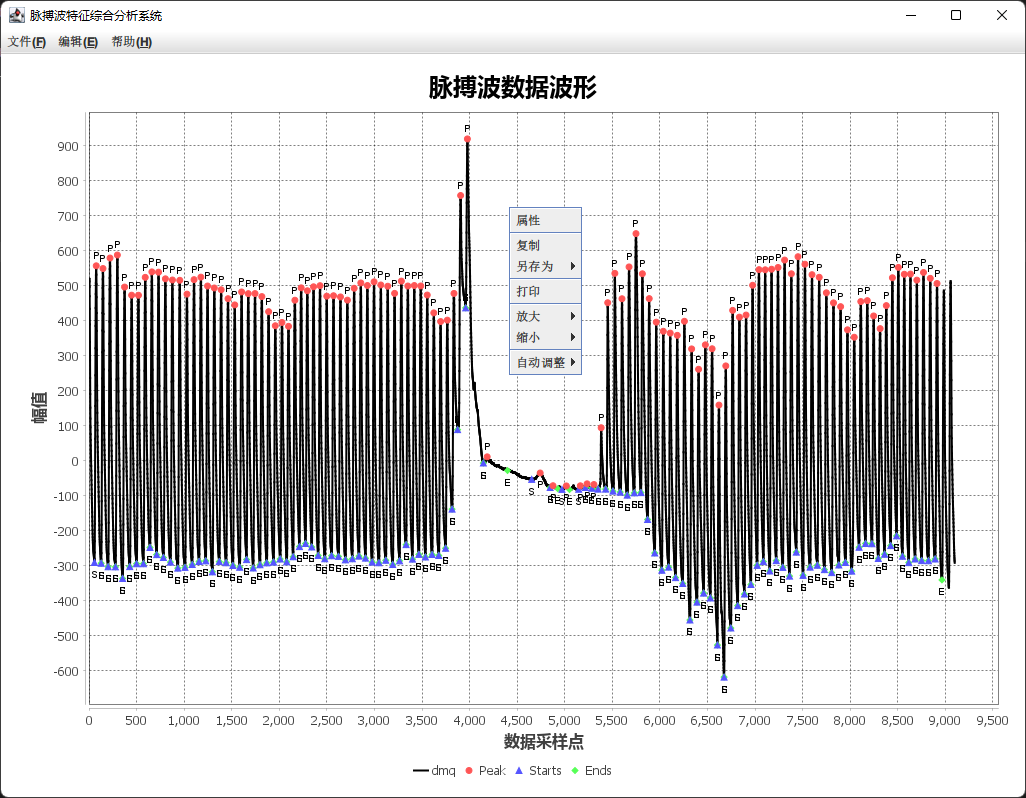
\includegraphics[width=.8\linewidth]{ch6/pc_ui}
%     \caption{\label{fig:pc_ui}PC软件运行界面}
% \end{figure}

2. Android界面

\autoref{fig:aui}展示了软件分析系统在Android上运行效果。
% \begin{figure}[htbp]
%     \centering
%     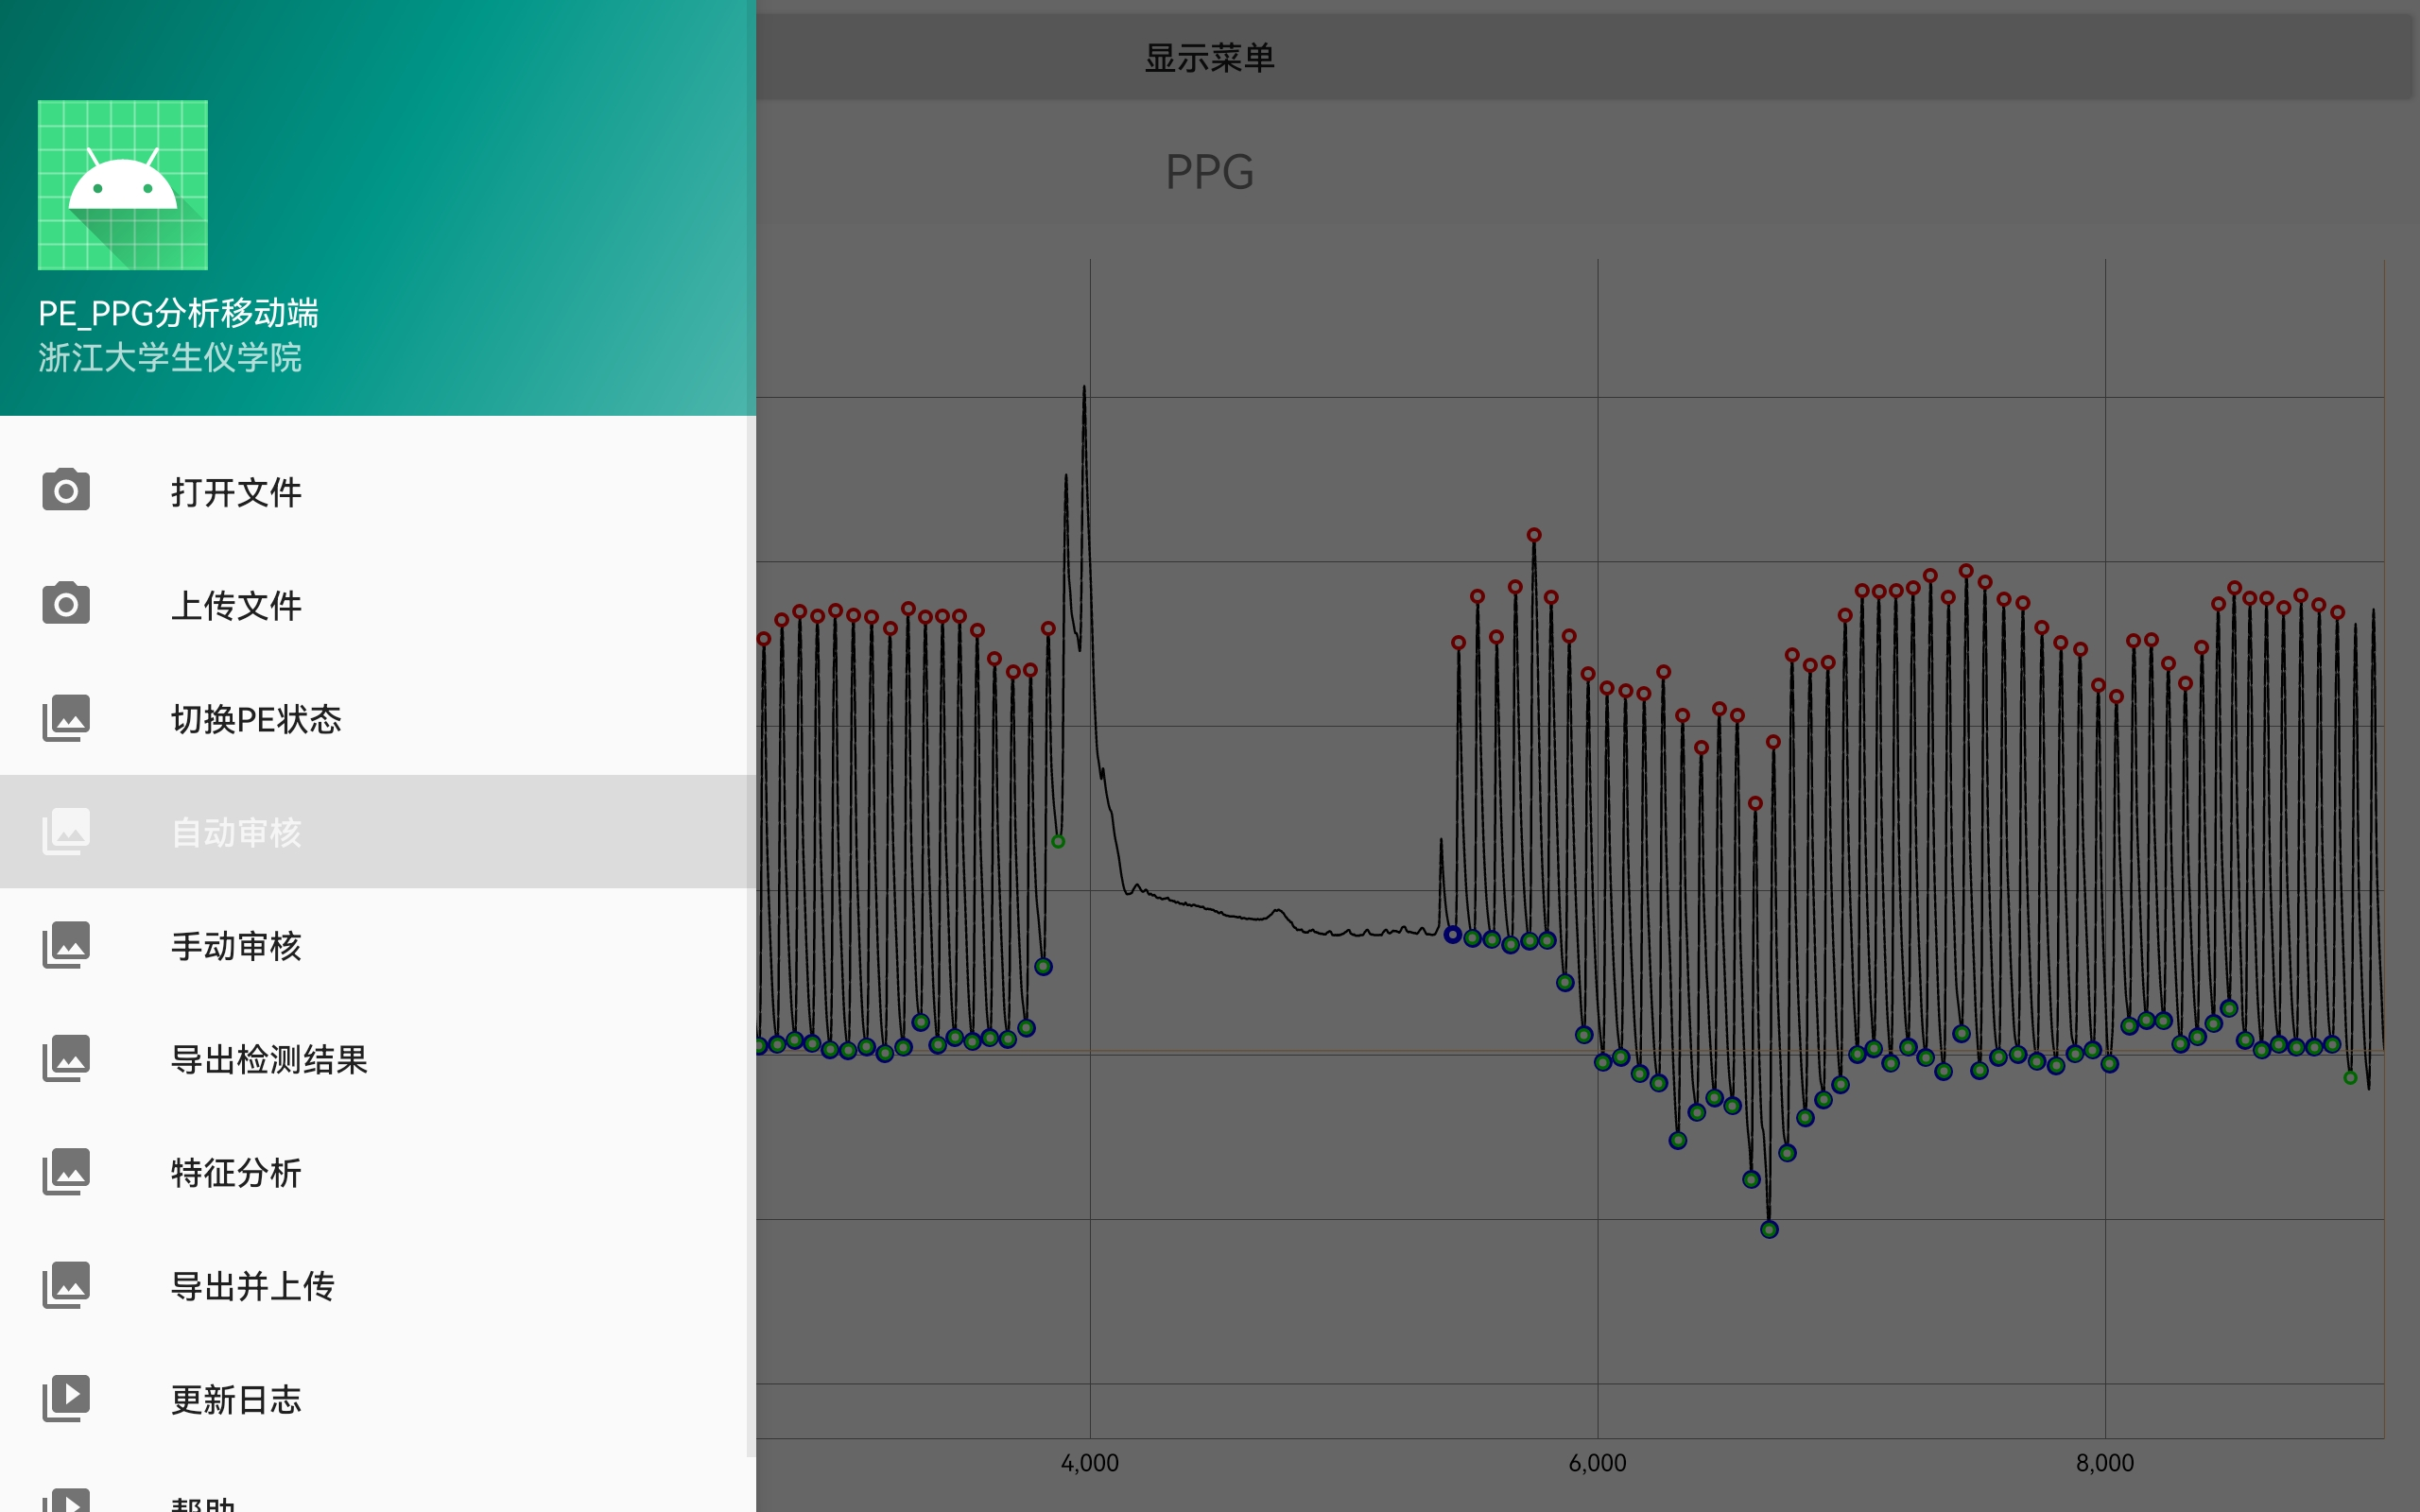
\includegraphics[width=.6\linewidth]{ch6/android_ui}
%     \caption{\label{fig:aui}Android软件运行界面}
% \end{figure}

\subsection{服务器模块}

一、数据库设计

二、模型存储设计

三、模型调用设计

\subsection{模型训练模块}
一、数据获取

二、模型训练

\section{系统验证与测试}
界面
输入输出
\section{小结}